    All the theory and algorithms presented in this section are
    defined and valid in arbitrary dimension $d$. They will however be
    illustrated in 2d for clarity, while experiments willl be
    performed on 3d digital shapes.  Let $\Z^d$ be the $d$-dimensional
    digital space.  Let $\mathcal{C}^d$ be the (cubical) cell complex
    induced by the lattice $\Z^d$ : its 0-cells are the points of
    $\Z^d$, its 1-cells are the open unit segments joining two 0-cells
    at distance 1, its 2-cells are the open unit squares, \ldots, and
    its $d$-cells are the $d$-dimensional open unit hypercubes with
    vertices in $\Z^d$.  We denote by $\mathcal{C}^d_k$ the set of its
    $k$-cells, for $0 \Le k \Le d$.  In the following, a cell always
    designates an element of $\mathcal{C}^d$, and the term subcomplex
    always indicates a subset of $\mathcal{C}^d$.

    The \emph{topological closure} of a cell $\tau$ is denoted by
    $\bar{\tau}$. The \emph{star} of a cell $\sigma$ is the subcomplex
    $\Star{\sigma}:=\{\tau \in \mathcal{C}, \sigma \subset \bar{\tau}
    \}$. It is naturally extended to any subcomplex $K$ by union,
    i.e. $\Star{K} := \cup_{\sigma \in K} \Star{\sigma}$, and more
    generally to any subset $Y$ of $\R^d$ as $\Star{Y}:=\{ c \in \C,
    \bar{c} \cap Y \neq \emptyset \}$. The \emph{body} $\|K\|$ of $K$
    is its realization in $\R^d$, i.e. $\|K\|:=\cup_{c \in K} c$. One
    can check that $\Star{K}=\Star{\|K\|}$, so these definitions are
    sound.

    %% A cell $\sigma$ is a face of another cell $\tau$ whenever $\sigma$
    %% is a subset of the topological closure $\bar{\tau}$ of $\tau$,
    %% written $\sigma \preccurlyeq \tau$.  Given any subcomplex K of
    %% $\mathcal{C}^d$, the star $Star(K)$ of K is $\{\tau \in
    %% \mathcal{C}^d, s.t.\ \exists\sigma \in K,\sigma \preccurlyeq
    %% \tau\}$.
    \begin{definition}[Visibility]
      Let $Z \subset \Z^d$ be a digital set. Two digital points $p$
      and $q$ are \emph{visible in $Z$} if and only if the straight
      segment $[p, q]$ is included in $\Star{Z}$, i.e., $\Star{[p, q]}
      \subseteq \Star{Z}$.
    \end{definition}
    This definition corresponds to the concept of tangency presented
    in \cite{lachaud:2022-jmiv}, limited to pair of points. One can
    check that $p$ and $q$ must belong to $Z$ to be visible.
    
    % Examples of visibility in 2D
    \begin{figure}[t]
      \centering
      \begin{tabular}{c@{~}|@{~}c@{~}|@{~}c@{~}|@{~}c}
  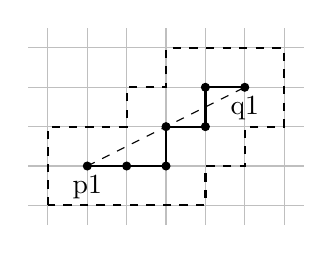
\begin{tikzpicture}
    \draw[step=0.5,lightgray,thin,xshift=-1cm,yshift=-1cm] (0.25,0.25) grid (3.75,2.75);
    \draw[dashed] (0,0) -- (2,1);
    \filldraw[black] (0,0) circle (0.05) node[anchor=north] {p1};
    \filldraw[black] (2,1) circle (0.05) node[anchor=north] {q1};
    \foreach \x/\y in {1/0,2/0,2/1,3/1,3/2} {
      \filldraw[black] (0.5*\x,0.5*\y) circle (0.05);
    }
    \draw [thick] (0,0) -- (0.5,0) -- (1,0) -- (1,0.5) -- (1.5,0.5) -- (1.5,1) -- (2,1);
    \draw[thick,dashed] (-0.5,-0.5) -- (-0.5,0.5) -- (0.5,0.5) -- (0.5,1) -- (1,1) -- (1,1.5) -- (2.5,1.5) -- (2.5,0.5) -- (2,0.5) -- (2,0) -- (1.5,0) -- (1.5,-0.5) -- (-0.5,-0.5);
  \end{tikzpicture} &
  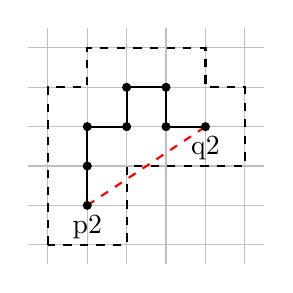
\begin{tikzpicture}
    \draw[step=0.5,lightgray,thin,xshift=-1cm,yshift=-1cm] (0.25,0.25) grid (3.25,3.25);
    \draw[red,dashed,thick] (0,0) -- (1.5,1);
    \filldraw[black] (0,0) circle (0.05) node[anchor=north] {p2};
    \filldraw[black] (1.5,1) circle (0.05) node[anchor=north] {q2};
    \foreach \x/\y in {0/1,0/2,1/2,1/3,2/3,2/2} {
      \filldraw[black] (0.5*\x,0.5*\y) circle (0.05);
    }
    \draw [thick] (0,0) -- (0,1) -- (0.5,1) -- (0.5,1.5) -- (1,1.5) -- (1,1) -- (1.5,1);
    \draw[thick,dashed] (-0.5,-0.5) -- (-0.5,1.5) -- (0,1.5) -- (0,2) -- (1.5,2) -- (1.5,1.5) -- (2,1.5)  -- (2,0.5) -- (0.5,0.5) -- (0.5,-0.5) -- (-0.5,-0.5);
  \end{tikzpicture} &
  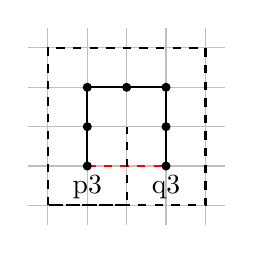
\begin{tikzpicture}
    \draw[step=0.5,lightgray,thin,xshift=-1cm,yshift=-1cm] (0.25,0.25) grid (2.75,2.75);
    \draw[red,dashed,thick] (0,0) -- (1,0);
    \filldraw[black] (0,0) circle (0.05) node[anchor=north] {p3};
    \filldraw[black] (1,0) circle (0.05) node[anchor=north] {q3};
    \foreach \x/\y in {0/1,0/2,1/2,2/2,2/1} {
      \filldraw[black] (0.5*\x,0.5*\y) circle (0.05);
    }
    \draw [thick] (0,0) -- (0,1) -- (1,1) -- (1,0);
    \draw[thick,dashed] (-0.5,-0.5) -- (-0.5,1.5) -- (1.5,1.5) -- (1.5,-0.5) -- (-0.5,-0.5) -- (0.5,-0.5) -- (0.5,0.5);
  \end{tikzpicture} &
  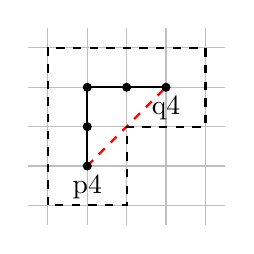
\begin{tikzpicture}
    \draw[step=0.5,lightgray,thin,xshift=-1cm,yshift=-1cm] (0.25,0.25) grid (2.75,2.75);
    \draw[red,dashed,thick] (0,0) -- (1,1);
    \filldraw[black] (0,0) circle (0.05) node[anchor=north] {p4};
    \filldraw[black] (1,1) circle (0.05) node[anchor=north] {q4};
    \foreach \x/\y in {0/1,0/2,1/2} {
      \filldraw[black] (0.5*\x,0.5*\y) circle (0.05);
    }
    \draw [thick] (0,0) -- (0,1) -- (1,1);
    \draw[thick,dashed] (-0.5,-0.5) -- (-0.5,1.5) -- (1.5,1.5) -- (1.5,0.5) -- (0.5,0.5) -- (0.5,-0.5) -- (-0.5,-0.5);
  \end{tikzpicture} \\
  Visible     & Non-Visible                   &
  Non-Visible & Non-Visible
\end{tabular}

%% \begin{tabular}{cc|cc}
%%   \begin{tikzpicture}
%%     \draw[step=0.5,lightgray,thin,xshift=-1cm,yshift=-1cm] (0.25,0.25) grid (3.75,2.75);
%%     \draw[dashed] (0,0) -- (2,1);
%%     \filldraw[black] (0,0) circle (0.05) node[anchor=north] {p1};
%%     \filldraw[black] (2,1) circle (0.05) node[anchor=north] {q1};
%%     \draw [thick] (0,0) -- (0.5,0) -- (1,0) -- (1,0.5) -- (1.5,0.5) -- (1.5,1) -- (2,1);
%%     \draw[thick,dashed] (-0.5,-0.5) -- (-0.5,0.5) -- (0.5,0.5) -- (0.5,1) -- (1,1) -- (1,1.5) -- (2.5,1.5) -- (2.5,0.5) -- (2,0.5) -- (2,0) -- (1.5,0) -- (1.5,-0.5) -- (-0.5,-0.5);
%%   \end{tikzpicture} & & &
%%   \begin{tikzpicture}
%%     \draw[step=0.5,lightgray,thin,xshift=-1cm,yshift=-1cm] (0.25,0.25) grid (3.25,3.25);
%%     \draw[red,dashed,thick] (0,0) -- (1.5,1);
%%     \filldraw[black] (0,0) circle (0.05) node[anchor=north] {p2};
%%     \filldraw[black] (1.5,1) circle (0.05) node[anchor=north] {q2};
%%     \draw [thick] (0,0) -- (0,1) -- (0.5,1) -- (0.5,1.5) -- (1,1.5) -- (1,1) -- (1.5,1);
%%     \draw[thick,dashed] (-0.5,-0.5) -- (-0.5,1.5) -- (0,1.5) -- (0,2) -- (1.5,2) -- (1.5,1.5) -- (2,1.5)  -- (2,0.5) -- (0.5,0.5) -- (0.5,-0.5) -- (-0.5,-0.5);
%%   \end{tikzpicture} \\
%%   Visible                       & & & Non Visible                   \\\\
%%   \hline\\
%%   \begin{tikzpicture}
%%     \draw[step=0.5,lightgray,thin,xshift=-1cm,yshift=-1cm] (0.25,0.25) grid (2.75,2.75);
%%     \draw[red,dashed,thick] (0,0) -- (1,0);
%%     \filldraw[black] (0,0) circle (0.05) node[anchor=north] {p3};
%%     \filldraw[black] (1,0) circle (0.05) node[anchor=north] {q3};
%%     \draw [thick] (0,0) -- (0,1) -- (1,1) -- (1,0);
%%     \draw[thick,dashed] (-0.5,-0.5) -- (-0.5,1.5) -- (1.5,1.5) -- (1.5,-0.5) -- (-0.5,-0.5) -- (0.5,-0.5) -- (0.5,0.5);
%%   \end{tikzpicture} & & &
%%   \begin{tikzpicture}
%%     \draw[step=0.5,lightgray,thin,xshift=-1cm,yshift=-1cm] (0.25,0.25) grid (2.75,2.75);
%%     \draw[red,dashed,thick] (0,0) -- (1,1);
%%     \filldraw[black] (0,0) circle (0.05) node[anchor=north] {p4};
%%     \filldraw[black] (1,1) circle (0.05) node[anchor=north] {q4};
%%     \draw [thick] (0,0) -- (0,1) -- (1,1);
%%     \draw[thick,dashed] (-0.5,-0.5) -- (-0.5,1.5) -- (1.5,1.5) -- (1.5,0.5) -- (0.5,0.5) -- (0.5,-0.5) -- (-0.5,-0.5);
%%   \end{tikzpicture}\\
%%   Non Visible (from a 1-d cell) & & & Non Visible (from a 0-d cell)
%% \end{tabular}

      \caption{Examples of visibility and non visibility in 2D within
        the set $X$ (represented with black disks $\bullet$).}
      \label{fig:visibility-2d}
    \end{figure}


    Figure~\ref{fig:visibility-2d} shows what is considered visible or not. We note that one particular aspect of this visibility definition is that all visible points from a given point taken as a separate complex are not necessarily 26-connected~\ref{fig:visibility-2d-not-connected}.
    Furthermore, we conjecture that they even may not be $n$-connected for $n$ arbitrarily large.
    This characteristic has implications for the applicability of Algorithm 3 from~\cite{lachaud:2022-jmiv}, as the algorithm assumes that visited points are 26-connected, potentially leading to incomplete collection of visible points.

    % Example of visibility not necessarily connected
    % Path from p to q : r u r u r r r r r u r
    \begin{figure}
        \centering
        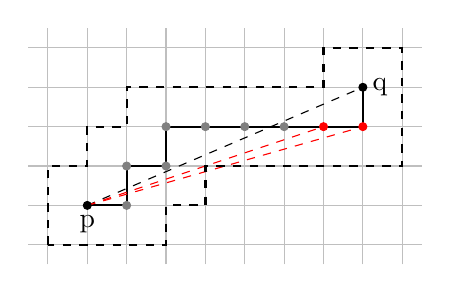
\begin{tikzpicture}
            \draw[step=0.5,lightgray,thin,xshift=-1cm,yshift=-1cm] (0.25,0.25) grid (5.25,3.25);
            \draw[thick] (0,0) -- (0.5,0) -- (0.5,0.5) -- (1,0.5) -- (1,1) -- (3.5,1) -- (3.5,1.5);
            \draw [black, dashed] (0,0) -- (3.5,1.5);
            \draw [red, dashed] (0,0) -- (3.5,1);
            \draw [red, dashed] (0,0) -- (3,1);
            \filldraw[black] (0,0) circle (0.05) node[anchor=north] {p};
            \filldraw[gray] (0.5,0) circle (0.05);
            \filldraw[gray] (0.5,0.5) circle (0.05);
            \filldraw[gray] (1,0.5) circle (0.05);
            \filldraw[gray] (1,1) circle (0.05);
            \filldraw[gray] (1.5,1) circle (0.05);
            \filldraw[gray] (2,1) circle (0.05);
            \filldraw[gray] (2.5,1) circle (0.05);
            \filldraw[red] (3,1) circle (0.05);
            \filldraw[red] (3.5,1) circle (0.05);
            \filldraw[black] (3.5,1.5) circle (0.05) node[anchor=west] {q};
            \draw[thick,dashed] (-0.5,-0.5) -- (-0.5,0.5) -- (0,0.5) -- (0,1) -- (0.5,1) -- (0.5,1.5) -- (3,1.5) -- (3,2) -- (4,2) -- (4,0.5) -- (1.5,0.5) -- (1.5,0) -- (1,0) -- (1,-0.5) -- (-0.5,-0.5);
        \end{tikzpicture}
        \caption{Example of non-connex visibility in 2D, q is visible from p while the visibility points are not 26-connected.}
        \label{fig:visibility-2d-not-connected}
    \end{figure}
